\section{Introduction}

In recent years, vector quantization (VQ) \cite{NIPS2017_7a98af17,NEURIPS2019_5f8e2fa1} has emerged as a foundational technique in unsupervised representation learning \cite{NEURIPS2020_92d1e1eb,pmlr-v235-bruce24a} and latent generative models \cite{Rombach_2022_CVPR,yu2022vectorquantized,yu2022scaling,10158503,wang2023neural,zhu-etal-2024-generative}. By converting continuous representations into discrete codes, VQ models can effectively identify the inherent structure of data and enable various discrete modeling methods on continuous data, from high-quality image generation \cite{Esser_2021_CVPR} to audio synthesis \cite{efossez2023high}. The recent success of Large Language Models (LLMs)~\cite{achiam2023gpt} has highlighted the effectiveness of next-token prediction as a powerful and versatile training objective. Consequently, VQ models are taken as the direct method to transform data from various modalities \cite{zhang-etal-2023-speechgpt,sun2024autoregressive,team2024chameleon} or scientific domains \cite{gao2024foldtoken} to discrete sequences for next token prediction training. However, attempts to integrate VQ models as multimodal tokenizers to leverage the scaling laws of LLMs face significant challenges because of the difficulty of expanding the codebook. For example, the Chameleon model \cite{team2024chameleon} constrains its codebook size to $8k$, which is significantly trailing behind the vocabulary size of LLMs (e.g., LLaMA3's vocabulary size is $128k$ \cite{dubey2024llama}).

\begin{figure*}[t]
    \centering
    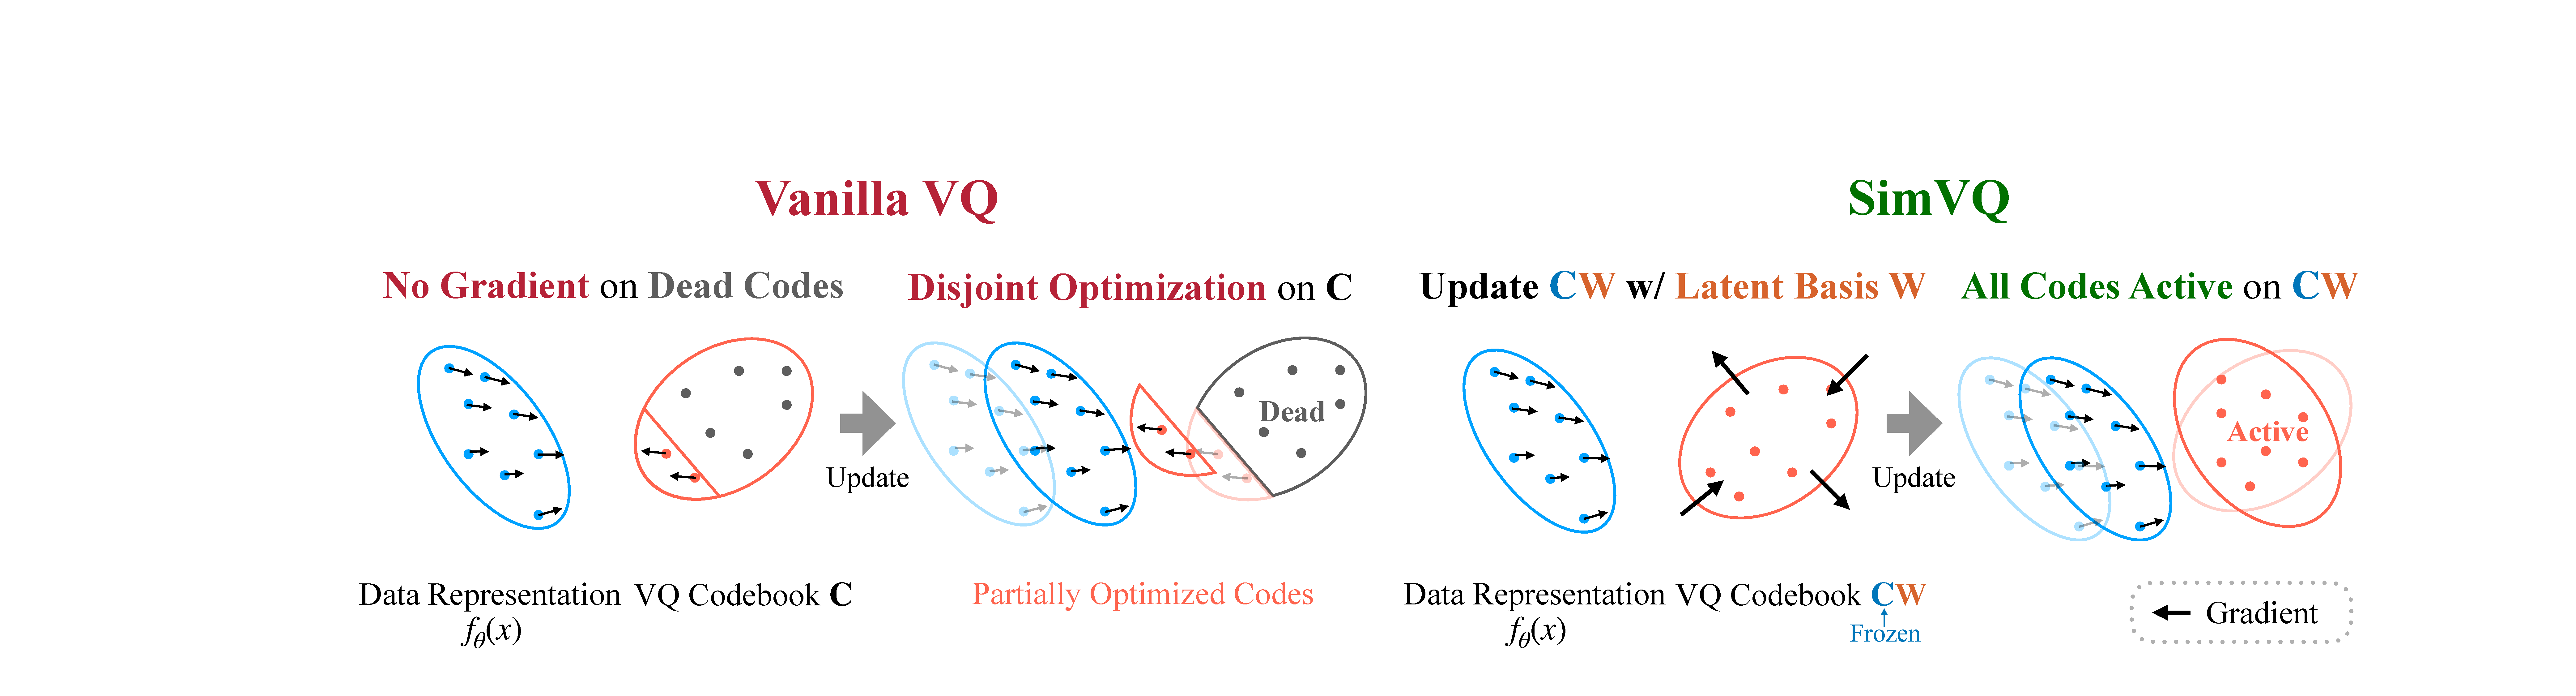
\includegraphics[width=2.0\columnwidth]{material/intro1_2_big.pdf}
    \caption{\textbf{Comparison of Vanilla VQ and SimVQ.} (a): (left) Disjoint optimization in Vanilla VQ. Only the nearest codes are updated, resulting in a high percentage of ``dead'' codes that are not updated. (b): (right) Joint optimization in SimVQ. The entire codebook is updated with a latent basis, ensuring all codes remain active.}
    \label{fig:intro}
\end{figure*}




There is a broad agreement that increasing vocabulary size can consistently improve the performance of LLMs \cite{tao2024scaling}. However, recent studies \cite{Zhu2024ScalingTC} indicate that traditional VQ models often fail to utilize the additional parameters introduced by codebook expansion, leaving most codes inactive during training. The contradiction between codebook expansion and low codebook utilization in VQ models is known as the representation collapse problem \cite{roy2018theory}, where increasing the codebook size fails to improve the performance. To address these discrepancies, we conduct a theoretical analysis of the optimization procedure of VQ models and identify that the disjoint optimization of the codebook is the root cause of representation collapse. As illustrated in Fig. \ref{fig:intro}(a), the core mechanism of VQ models involves a nearest-neighbor replacement strategy, where the encoder’s output features are replaced by the nearest vector in the codebook to serve as input to the decoder. The indices of the nearest vector are taken as the discrete representation of the data. This nearest-selection operator results in only a subset of codes being updated through gradient descent, while the remaining codes remain unchanged. 


Some methods mitigate representation collapse by hand-designing complex optimization strategies, such as stochastic quantization \cite{pmlr-v162-takida22a}, distribution penalty \cite{VQWasserstein,Xiao2023SCVAESC}, and codebook reset \cite{zheng2023online} through sophisticated training strategies. 
Recently, some approaches \cite{yu2022vectorquantized,mentzer2024finite,yu2024language} propose to reduce the dimension of the latent space to a very small scale (e.g., 8 v.s. 128) to alleviate the curse of dimensionality, thereby improving the overlap between the encoder’s features and the codebook. However, while these methods enhance codebook utilization, they do so at the cost of model capacity, leading to worse performance compared to vanilla VQ models when the codebook size is small or representation collapse is not severe. Another approach, VQGAN-LC \cite{Zhu2024ScalingTC}, initializes the codebook with features extracted from the pre-trained CLIP model \cite{pmlr-v139-radford21a} to create a well-structured latent space that better matches the distribution of the encoder output. Nevertheless, the latent space defined by an external pre-trained model limits the model's ability to generalize to diverse datasets and reaches a performance plateau as the codebook size increases. These limitations highlight the need for a more effective method to improve codebook utilization without compromising model capacity or relying on external models.


We critically assess prevalent methodologies and reveal that optimizing the latent space rather than individual code vectors is key to preventing representation collapse. Building on this insight, we introduce a simple yet effective method, termed SimVQ, to directly update the latent space spanned by the codebook by linear transforming the code vectors via a learnable latent basis. Specifically, the vectors in the codebook are reparameterized as a linear combination of the basis in the learnable linear layer $\bm{W}$:
\begin{equation}
    \bm{C} \in \mathbb{R}^{K\times d} \Rightarrow \bm{CW} ~\text{with}~ \bm{W} \in \mathbb{R}^{d\times d},
\end{equation}
where $K$ denotes the codebook size and $d$ represents the dimension of latent space. This reparameterization with linear transformation disentangles the optimization of the codebook into two components: the coefficient matrix $\bm{C}$ and the basis of linear space $\bm{W}$ respectively. As illustrated in Fig. \ref{fig:intro}(b), by optimizing the basis matrix $\bm{W}$, the latent space spanned by $\bm{CW}$ is rotated and stretched to match encoder's output feature. The entire codebook is updated jointly to prevent the representation collapse problem. The simplicity of the proposed method makes it highly portable and easily adaptable for improving VQ-based models across a wide range of domains, requiring only \textit{one linear layer}.


In summary, our contributions to vector quantized models are as follows:
\begin{itemize}
    \item We theoretically analyze the representation collapse problem in VQ models and reveal that optimizing the latent space spanned by the codebook, rather than individual code vectors, is crucial to addressing this issue. 
    \item We propose a novel method, SimVQ, which reparameterizes the codebook vectors in VQ models via a linear transformation with a learnable latent basis. This simple yet effective approach is highly adaptable and easy to implement, making it broadly applicable across various machine learning contexts.
    \item We conduct an extensive evaluation of SimVQ across diverse modalities, including image and audio with different model architectures. The results show that SimVQ not only effectively addresses the representation collapse problem by achieving near-complete codebook utilization regardless of the codebook size, but also establishes new state-of-the-art performance. Furthermore, when scaling up the codebook size, SimVQ consistently delivers improved results.
\end{itemize}
